\chapter{Background}

In this chapter we describe the background necessary to understand the work that follows. We first introduce what can now be considered “classical” Reinforcement Learning and its mathematical formalization as a Markov Decision Process. 
\\\\
We then introduce Artificial Neural Networks (ANN) - a key concept in all of modern Machine Learning (which RL is a subset of). In particular, we will see that at their core, ANNs are simply non-linear function approximators. Additionally, we look at Convolutional Neural Networks (CNNs) - a special type of ANNs that performs well on data containing spatial information, such as images. 
\\\\
Combining RL with ANNs we arrive at Deep Reinforcement Learning (DRL) and describe the relatively novel algorithm used in this thesis: Advantage Actor-Critic. We will then briefly describe some successful applications of RL algorithms to various games. Finally, we will describe StarCraft II video game, its rules, and the DeepMind’s PySC2 library through which communication with StarCraft II is made.

\section{Reinforcement Learning}

The idea of learning by reinforcement is historically rooted in behavioral psychology~\cite{Thorndike1898}, and boils down to the observation that an animal is more likely to repeat a desired pattern of actions in a given environment if the actions are followed by a stimulus (either positive or negative). Applying this idea to the context of self-learning agents in computer science, the field of Reinforcement Learning was formed~\cite{Samuel1959}.
\\\\
A typical RL model describes an agent taking actions in some environment and receiving rewards (typically scalar values) as a result (see Figure~\ref{fig:mdp}). The goal of the agent is to find best choice of actions for every given state such that agents returns (cumulative rewards) are maximized.
\\\\
For example, in the classical game of Tic-Tac-Toe, the agent navigates $3\times3$ board states by choosing actions from a list of available cells, receiving $+1$ for a winning move (with $-1$ to the opponent) and $+0.5$ for a tie.
\\\\
There is no direct control over the specifics of the learned behavior, which are left for the agent to decide as long as it satisfies the goal of maximizing returns. This is in contrast with the more common Supervised Learning based approaches, where the researcher provides the agent with samples of state and optimal action pairs, typically collected by observing human experts. 

\begin{figure}[ht]
\begin{center}
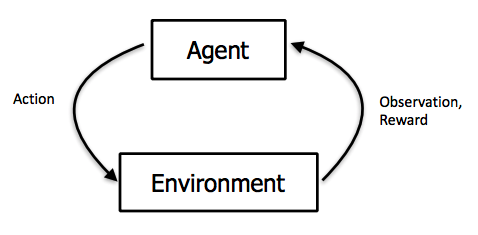
\includegraphics[width=0.8\textwidth]{mdp}
\caption[]{Reinforcement Learning model of interaction with the environment.\\\small{Source: CS294 DRL Course, Berkeley \url{http://rll.berkeley.edu/deeprlcourse-fa15} } }
\label{fig:mdp}
\end{center}
\end{figure}

\noindent Autonomy of learning agents in RL based approaches is the reason they are often considered to be closest to human intelligence and a potential key to eventually solving the problem of Artificial General Intelligence (AGI) -- an AI capable of conscious thought and reasoning.
\\\\
While the end goal of RL may lie in practical applications such as optimization of data center energy consumption~\cite{Gao2014} or even as grandiose as solving AGI, there is a need for simpler environments to initially test novel approaches. 
As the field evolved, games quickly became the benchmark environments of choice for many researchers as they are defined with (relatively) simple rules for navigation (ex. move up or down) and clear reward signals (ex. win or lose). 
\\\\
In fact, the birth of RL field is often linked to an early AI experiment with a self-learning agent that quickly surpassed its creator at the game of checkers~\cite{Samuel1959}. This at the time monumental success for the AI field had the unfortunate side-effect of cultivating too much interest from the general public. The interest peaked with the release of Marvin Minsky's ``Perceptrons'' book, but eventually lead to (understably) failed expectations and the so-called ``AI winter''.
\\\\
Problems of unreasonable expectations haunt the field of AI to this day, fueled now more so by fear of ``Terminator''-like events, where a sentient AI chooses to eliminate the human race based on incorrectly provided reward function. It is important to consider the possibility of such events, and discuss ways to build in safety measures, but RL as a field is still in very early stages and it is more productive to focus on development and improvement of RL based approaches based on game environments.
\\\\
Reinforcement Learning algorithms are often divided into model-based and model-free categories. Model-based algorithms attempt to learn a model of the environment, represented by the transition probabilities and reward function in the MDP formulation above. In contrast, model-free RL algorithms focus only on the end goal of cumulative reward maximization, effectively disregarding information about the environment the agent is operating in. While there are pros and cons to both approaches, RL researchers mainly focused on model-free algorithms due to their relative simplicity in implementation and computation. For simplicity, all the work that follows is implicitly assumed to be in the model-free RL family.
\\\\
The two dominant approaches to solving Reinforcement Learning problems in a model-free fashion are defined by the underlying optimization problem they are solving: either by optimizing on the expected value of the actions (e.g. Q-Learning) or on the policy itself (e.g. Policy Gradients). These approaches are different enough to have evolved into two separate families of algorithms and are explored in greater detail in sections \ref{vbm}, \ref{pbm} below.
\\\\
While there are many different approaches to solving RL based problems, one common thing between them all is in their mathematical formalization as a Markov Decision Process.

\subsection{Markov Decision Process} \label{mdp}

The problem of RL can be viewed as a Markov Decision Process (MDP), which is formally defined by the $<S,A,P,R>$ tuple:

\begin{itemize}
\item S: set of all possible states
\item A: set of all possible actions
\item P: $(S,A,S) \rightarrow [0,1]$, where $P(s'|s, a)$ is the probability of arriving at $s’ \in S$ given $s \in S$ and $a \in A$
\item R: $(S,A,S) \rightarrow \mathbb{R}$, where $R(s, a, s')$ is the reward function for arriving in state $s' \in S$, while taking action $a \in A$ in state $s \in S$
\end{itemize}

\noindent That is, given a set of all possible states $S$, a set of all possible actions $A$, transition probability function $P$, and a reward function $R$, find an optimal policy $\pi$ -- probability distribution over action space given current state -- such that expected returns are maximized. Policy can be either deterministic $\pi(s)$ or stochastic $\pi(a|s)$.
\\\\
The underlying stochastic process is defined by the transition probability $P$ and in the context of RL problems (especially in games) is often implicitly assumed to be stationary, meaning it does not change over time. This assumption significantly simplifies following theoretical reasoning about the agent.
\\\\
As the agent acts in the same environment with discrete timesteps, it is often useful to reason about the sequence of states, actions and rewards through time together as a single trajectory $\tau$: $<s_0, a_0, r_1>, <s_1, a_1, r_2>, \dots, <s_{n-1}, a_{n-1}, r_{n}>$, where $r_t$ represents agents immediate reward at a given time-step $t$: $r_t = R(s_{t-1}, a_{t-1}, s_{t})$.
\\\\
If full state information is not accessible to the agent then it is possible to extend definition above and model the problem as a Partially Observable Markov Decision Process (POMDP), which defines an additional observation set $O$ and its conditional probabilities $P_O(o | s', a)$.

\subsection{Credit Assignment Problem}

% TODO cite Minsky, 1963
While an agent receives some rewards immediately after an action was taken, it is often unclear whether the action actually contributed to the reward gained. Imagine a game of Tic-Tac-Toe where the agent has caught the opponent in a trap which will lead to his inevitable loss. While the win reward will be assigned to the final action, the contributing action was actually made beforehand. This is known as credit assignment problem and it is an open area of research.
\\\\
% TODO cite
One very common solution to the credit assignment problem is known as  n-step discounted returns, where the cumulative rewards following action $a_t$ for $n$ steps are exponentially weighted by some $\gamma \in (0, 1]$:

$$R_t = \sum\limits_{k=0}^n \gamma^k r_{t+k+1}$$

\noindent The task is to then find an optimal policy $\pi$ that maximizes expected returns $\mathbb{E}_{s_{t+1} \sim P(\cdot|s_t,a_t), a_t \sim \pi(s_t)}[R_t|s_t = s]$ for all $s \in S$.

\subsection{Value-Based Methods} \label{vbm}

In value-based RL methods the goal of finding an optimal policy $\pi(s)$ is defined through maximizing the estimate the state value function: 

$$V_\pi(s) = \mathbb{E}_{s_{t+1} \sim P(\cdot|s_t,a_t), a_t \sim \pi(s_t)}[R_t|s_t = s]$$

\noindent However, this task is not possible to solve in most real-world applications as we do not know the transition probabilities. For this reason the notion of state-action pair $Q_\pi(s,a)$ (Q-value) is introduced and optimized instead:

$$Q_\pi(s_t,a_t) = \mathbb{E}_{s_{t+1} \sim P(\cdot|s_t,a_t)}[R_t|s_t = s, a_t = a]$$

\noindent Q-value represents expected cumulative reward given that action $a \in A$ is taken in state $s \in S$, followed by actions chosen based on the policy $\pi$. It is often more useful to define Q-value recursively, separating immediate reward to its own component:

$$Q_\pi(s_t, a_t) = \mathbb{E}_{s_{t+1} \sim P(\cdot|s_t,a_t)}[R(s_t, a_t, s_{t+1}) + \gamma Q_\pi(s_{t+1}, a_{t+1})]$$

\noindent Recursive definition above is commonly refered to as the Bellman Equation and is tightly related to the Bellman Optimality Equation:

$$Q^*(s_t, a_t) = \mathbb{E}_{s_{t+1} \sim P(\cdot|s_t,a_t)}[R(s_t, a_t, s_{t+1}) + \gamma \max\limits_{a_{t+1}}Q^*(s_{t+1}, a_{t+1})], $$

\noindent where $Q^*(s, a)$ denotes an optimal state-action value function. This definition has a favorable property -- it can be iteratively approximated (by e.g. bootstrapping). There are several algorithms based on this definition, one popular among them is the Q-Learning algorithm~\cite{Watkins1992}.
\\\\
The Q-Learning algorithm approximates optimal state-action values $Q^*(s, a)$ with Temporal Difference (TD) Learning, a general framework for iteratively optimizing a function while bootstrapping from current estimates~\cite{Sutton1988}. In context of Q-Learning, the TD update step is defined as follows ($\alpha$ is learning rate):

$$Q_{i+1}(s_t, a_t) \leftarrow Q_{i}(s_t,a_t) + \alpha\big(r_{t+1} +  \gamma \max\limits_{a}Q_{i}(s_{t+1}, a) - Q_{i}(s_t, a_t)\big)$$

\noindent This algorithm is guaranteed to produce an optimal greedy policy $\pi(s) = \argmax\limits_a Q(s,a)$.
\\\\
In practice, learned policy is often parametrized by some set of parameters $\theta$. Though in that case convergence guarantees do not hold, empiricially this has proven not to be an issue in most RL based problems.

\subsection{Policy-Based Methods} \label{pbm}

Alternative approach to value-based methods is to directly optimize the parametrized policy $\pi(a|s;\theta)$ with regards to the expected returns $\mathbb{E}_{s_{t+1} \sim P(\cdot|s_t,a_t), a_t \sim \pi(s_t)}[R_t|s_t = s]$. There are several reasons why this approach could be beneficial or even the only viable option, for example continuous action space or a need for stochastic policy.
\\\\
In policy-based methods the optimization procedure is typically done with gradient descent family of algorithms. There are several ways to define the cost function for the underlying optimizer, but by far the most common method is the REINFORCE family~\cite{Williams1992}.
\\\\
The core of the REINFORCE approach is in its unbiased re-parametrization of the optimization target which results in their gradients definition being computationally feasible for stochastic optimization procedure. Specifically, REINFORCE defines an unbiased estimate of $\nabla_{\theta} \mathbb{E}[R_t|s_t]$ as $\nabla_{\theta} \log \pi(a_t|s_t;\theta)R_t$~\cite{Williams1992}.

\subsection{Actor--Critic Methods}

REINFORCE approach can be improved by reducing variance of the gradient estimate with a baseline $b_t(s_t)$ subtracted from the returns $R_t$, resulting in the estimate $\nabla_{\theta} \mathbb{E}[R_t|s_t]$ taking the form $\nabla_{\theta} \log \pi(a_t|s_t;\theta)(R_t - b_t(s_t))$, which is shown to remain unbiased~\cite{Williams1992}.
\\\\
Often used baseline is an estimate of the state value function $V_\pi(s) = \mathbb{E}[R_t|s_t = s]$. Since $R_t$ can be shown to be an estimate of $Q_\pi(s, a) = \mathbb{E}[R_t|s_t = s, a_t = a]$, then $R_t - V_\pi(s_t)$ can be considered to be an estimate of the advantage function $A(s_t, a_t) = Q_\pi(s_t, a_t) - V_\pi(s_t)$.
\\\\
Algorithms that learn with the resulting estimate $\nabla_{\theta} \log \pi_{s_t}(a_t;\theta)\hat{A}(s_t, a_t)$ are referred to as the Actor-Critic methods, with the idea of the approach boiling down to the combination of optimization targets of the policy (actor) and the value (critic) terms~\cite{Sutton1998}. See Figure~\ref{fig:ac} below for a visual model.
\\\\
Intuitively this approach can be understood as agents inner dialogue where the agent learns to act optimally in his environment, while scrutinizing his behavior based on the missed expected returns.
\\\\
Though the critic terms name and its relation to Q-Learning can be deceiving, as critic’s task is not so much tied to agents ability to navigate the environment as it is to accurately predicting the value of the current state. 
%This in turn means that from critic’s perspective, the optimal behavior could be to remain motionless, as the agent can then effortlessly predict the value of the state.

\begin{figure}[ht]
\begin{center}
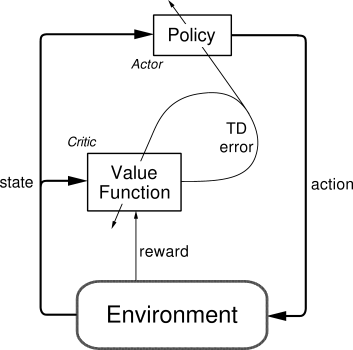
\includegraphics[width=0.5\textwidth]{ac}
\caption{Actor-Critic model as illustrated in~\cite{Sutton1998}.}
\label{fig:ac}
\end{center}
\end{figure}

\section{Function Approximation}

While an RL agent can be successfully trained on full state representations when the state space is relatively simple, the problem quickly becomes computationally infeasible as the state dimensionality and complexity grows. For this reason, a function approximator is often used that serves both as a dimensionality reduction technique and the mapping of similar states to the same result. 
\\\\
Though it should be noted that by using function approximators, convergence guarantees are not necessarily going to hold. In practice however that is rarely a significant problem. In particular, a staple of modern RL algorithms has become the use of a specific type of non-linear function approximators, commonly referred to as Artificial Neural Networks.

\subsection{Artificial Neural Network}

As the name suggests, Artificial Neural Networks are inspired by neuronal connections in the brain. The idea of using brain-inspired mathematical models was first explored relatively long ago~\cite{McCulloch1943}, but it only really took off with introduction of backpropagation: a method to iteratively calculate derivatives of complex functions by applying dynamic programming techniques~\cite{Rumelhart1986}. 
\\\\
In practice, the backpropagation procedure is typically done behind the scenes by automatic differentiation libraries such as TensorFlow~\cite{Abadi2016} or PyTorch~\cite{Paszke2017}.
\\\\
Formally, ANNs can be viewed as non-linear function approximators:

$${\hat f(x)} = W_nh_n(W_{n-1}h_{n-1}(\dots(W_0x + b_0)\dots) + b_{n-1}) + b_n,$$

\noindent where $h_i(x)$ is the activation function -- a function that ensures non-linearity in the approximator at layer $i$. It was shown that with the correct choice of the activation function, ANNs are able to approximate any continuous function in a compact subset of $\mathbb{R}^n$, making them universal approximators~\cite{Hornik1991}. Typical examples of $h(x)$ are $sigmoid$ and $tanh$.
\\\\
While $sigmoid$ and $tanh$ were favorable mathematically, having desirable properties such as continuity and differentiability, they also resulted in convergence breaking side-effects such as “vanishing” gradients, where the gradient of the function quickly became zero as the input grew in magnitude. Recently, Rectified Linear Unit (ReLU, $h(x) = max(0, x)$) became the nonlinearity function of choice for many researchers as it doesn’t suffer from vanishing gradient problems, and is computationally faster~\cite{Nair2010}. 
\\\\
ANNs enjoyed some success during 1980-1990, a notable example of that would be “ALVINN” - an automated vehicle where turning direction was chosen by the ANN~\cite{Pomerleau1989}. But their real potential was showcased only in second part of 2000s, when people started experimenting with running massively parallel matrix computations on specialized hardware, most notably on easily accessible consumer graphics processing units by NVIDIA.
\\\\
This, coupled with practical advancements in model initialization~\cite{Hinton2006}, led to breakthroughs in many areas. Notably, in 2012 this led to significant improvements over state-of-the-art at the time in speech recognition~\cite{Dahl2012} and in image recognition~\cite{Krizhevsky2012}, the latter was done by making use of a special type of layer, specialized for spatial information processing -- convolutional layer.

\subsection{Convolutional Neural Network}

% TODO cite text
Convolutional Neural Networks are a special type of ANN that contain one or more convolutional layers. These layers are designed to work well on certain types of data such as images, making use of the inherent spatial information while keeping number of parameters relatively small (compared to classical ANNs). While used mainly for image processing, they have been recently shown to perform well on text-based tasks as well.
\\\\
Each layer consists of a number of filters: small tensors, typically $3 \times 3 \times C$ or $5\times 5 \times C$ in size (where $C$ matches the image depth), that produce outputs by performing sliding window dot products on localized parts of the input image step-by-step (Figure~\ref{fig:cnn}). Step size (or stride) is often fixed to 1 (meaning sliding window moves 1 pixel at a time), although other options are also not uncommon. Sometimes image dimensions will not be compatible with configured filter size and stride in which case input image border is often padded with zeros as a workaround. 
\\\\
The idea of using convolutional layers on spatial information has been explored in the past~\cite{Fukushima1980}, but the biggest showcase of their potential was probably done by “AlexNet” - a specialized ANN architecture that has won ImageNet Large Scale Visual Recognition Challenge in 2012 with a significant jump in classification accuracy performance~\cite{Krizhevsky2012}. This achievement is often referred to as the start of “Deep Learning” era in Machine Learning.

\begin{figure}[ht]
\begin{center}
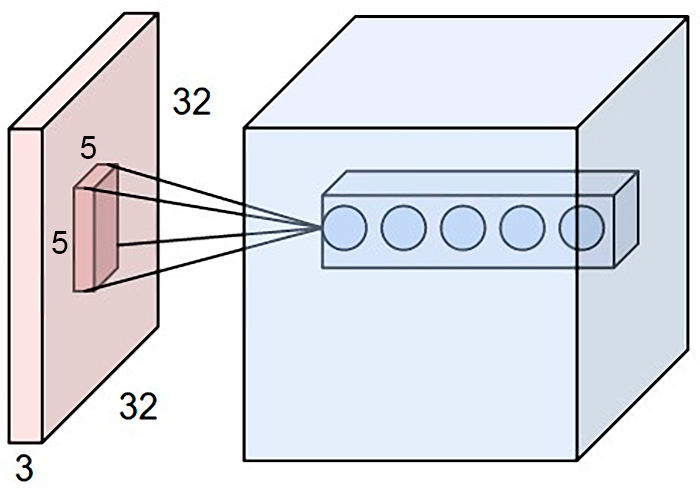
\includegraphics[width=0.8\textwidth]{cnn}
\caption{Convolutional layer. Each circle represents a single filter of size $5\times 5 \times 3$. Here the first filter is performing a dot product on the middle portion of the input image.
Source: \url{http://cs231n.github.io/convolutional-networks/} }
\label{fig:cnn}
\end{center}
\end{figure}

\noindent\\ CNN based architectures are particularly notable because they are first examples of “end-to-end” solutions, where a single Artificial Neural Network performs all the necessary sub-tasks for problems such as recognition and classification. Prior to CNNs, typical image processing solutions contained multitude of hand-crafted filters and input preprocessing functions, all of which often required domain experts to write. Though some researchers argue that relying on convolutional layers in itself can be considered domain knowledge and thus CNN based approaches cannot be called truly “end-to-end”.

\section{Deep Reinforcement Learning}

Using Artificial Neural Networks as function approximators for classical RL algorithms has led to a significant improvement in their performance across many different tasks and environments. This has put the field of Reinforcement Learning into the spotlight both for researchers and the general public. 
\\\\
The idea itself was not novel and first successful applications date as far back as 1995 with TD-gammon: a Backgammon AI that relied on NNs for state evaluation~\cite{Tesauro1995}. But the work that has led to bringing RL approaches notoriety is most likely to be DeepMind’s Atari AI. 
\\\\
DeepMind researchers showed the full potential of RL based approaches with their Deep Q-Network paper, which used Atari Learning Environment -- an emulator for the classical Atari console video games -- as their benchmark environment. The importance of this paper was in the fact that the agent was learning to outplay human experts by learning only from the raw pixel inputs, not only resembling how a human would perceive the game, but also not having access to any domain knowledge from the experts~\cite{Mnih2015}.
\\\\
This was the first time an AI agent was capable of surpassing human performance in a complex environment while having no additional information such as domain specific features, and has led to an explosion in research of (Deep) Reinforcement Learning based approaches. 

\subsection{Advantage Actor-Critic (A2C)}

The algorithm known as A2C has an interesting history of conception in that there is no official publication describing it, even though it is widely used and referenced.
\\\\
In articles, A2C is often defined as a synchronous version of the Asynchronous Advantage Actor-Critic (A3C) algorithm~\cite{mnih16}. The two algorithms are essentially equivalent mathematically, though this is not the case when it comes to technical implementation.
\\\\
Conceptually the A2C/A3C algorithms are quite similar to the classical actor-critic methods described in section 1.1.5, where the policy $\pi_s$ (actor) and value estimate $V_\pi(s)$ (critic) are trained at the same time as a form of self-scrutinizing learning loop. However, there are some key differences that are big enough to warrant considering them as a separate algorithm.
\\\\
First, the use of Neural Networks as end-to-end non-linear function approximators both for the value and policy outputs. This breaks any convergence guarantees provided by the original algorithms, but significantly improves the level of complexity of environments an agent can learn to navigate in.
\\\\
Second, the algorithms' key selling point is in their capacity for mass parallelization. For A3C this is defined through client-server architecture, where each client contains a local copy of the model, computes its own gradients and pushes those to the central server. Central server performs a single optimization step based on the incoming gradients, updates model weights (parameters of the ANN) and then distributes new model version to all child workers. 
\\\\
In A2C, everything related to the model is stored on the server side, with client workers are only responsible for communicating with the environment itself. A2C workers are executed synchronously, which results in a trade-off between performance during sample gathering stage and during training stage. A2C gains significant computational speed due to the fact that the model can be efficiently executed on the GPU hardware, which is in contrast with the typically CPU only architecture of A3C based agents.
\\\\
Finally, a common pitfall of the original actor-critic algorithms is the exploration/exploitation problem, which refers to maintaining a healthy balance between greedily following the current best policy (exploitation) and experimenting with alternative policies to see if the result improves (exploration). Since both policy and value functions are parametrized and are not guaranteed to converge to optimal values, an agent can quickly converge to some local optimum which may be far from desired behavior. 
\\\\
In the A2C/A3C algorithms this problem is alleviated by introducing a separate policy entropy maximization target to the gradient descend optimization objective. Specifically, the optimization problem is solved with the additional entropy term.
\\\\
The full objective loss function for some sampled trajectory $\tau$ is defined as follows:

$$J(\theta) = \mathbb{E}_{\tau} \bigg[\log \pi(a_t|s_t;\theta)\hat{A}(s_t, a_t) + \big(R_t - \hat{V}(s_t;\theta) \big)^2  - \pi(a_t|s_t;\theta) \log(\pi(a_t|s_t;\theta))\bigg]$$

\noindent We can now present pseudo-code for the described Advantage Actor-Critic algorithm, roughly adapted from~\cite{mnih16}:

\begin{algorithm}
\caption{Advantage Actor-Critic algorithm}
\begin{algorithmic}
\State \textbf{input:} learning rate $\alpha$, number of updates $T_{max}$, number of n-steps $t_{max}$
\While {$T < T_{max}$}:
  \State $t \leftarrow 0$
  \State Get $s_0$ state
  \While {$t < t_{max}$}:
    \State Perform $a_t \sim \pi(\cdot|s_t;\theta)$
    \State Get $r_t$ reward and $s_{t+1}$ state
    \State $t \leftarrow t + 1$
  \EndWhile
  \If {$s_{t-1}$ is not terminal}:
    \State $R_{t_{max}} \leftarrow \hat{V}(s_{t-1};\theta)$
  \Else
    \State $R_{t_{max}} \leftarrow 0$
  \EndIf
  \ForAll {$i \in \{t_{max}-1, \dots, 0\}$}:
    \State $R_i \leftarrow r_i + \gamma R_{i+1}$
  \EndFor
  \State $\theta \leftarrow \theta + \alpha \nabla_{\theta} J(\theta)$
  \State $T \leftarrow T + 1$
\EndWhile
\end{algorithmic}
\end{algorithm}

\section{StarCraft II}

StarCraft was an immensely popular video game developed and published by Blizzard Entertainment in 1998. Much like the classical board games such as chess and go, StarCraft holds the property of being relatively easy to learn, but extremely difficult to master. This ensured that interest in the activity is not quickly lost and, given competitive nature of humans, eventually led to a competitive following. Many consider StarCraft as one of the contributing games to the birth of the e-sports movement.
\\\\
In fact, this game was considered a national sport of South Korea for almost two decades with many young people pursuing professional careers as StarCraft players, joining one of many organizations that specialized in this sport. Major tournaments were broadcasted live on television and gathered millions of viewers. Best players in South Korea were often very well-paid and recognized by the general public on same level as celebrities and athletes in more traditional sports. % (Figure \ref{fig:spl})

%\begin{figure}[ht]
%\begin{center}
%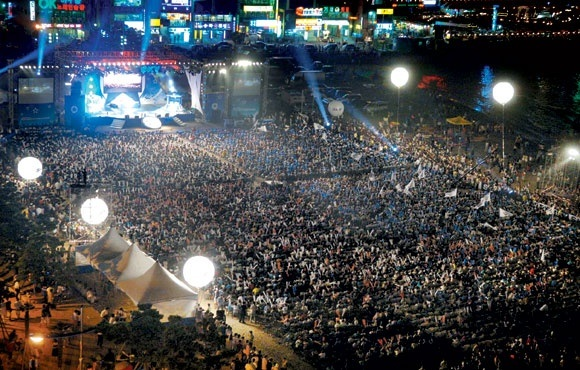
\includegraphics[width=\textwidth]{spl}
%\caption{Aerial view of the 2004 StarCraft Proleague Finals tournament with over 100,000 people in attendance.}
%\label{fig:spl}
%\end{center}
%\end{figure}

\noindent \\ However, given rapid technological advancement, StarCraft started to become outdated and in 2010 Blizzard released its successor StarCraft II. While not as popular as its ancestor due to rise of many great competitors, it still gathers thousands of viewers for regular tournaments broadcasted live of various platforms.
\\\\
The fact that this game is still played actively by millions of people across all levels of expertise from amateur beginner to professional veteran is very important from the point of view of AI research. Given that humans are still the best known solvers of complex and abstract tasks, they can play roles of a benchmarks for AIs and provide demostrations for the AI agents to learn from.
\\\\
StarCraft II is a real-time strategy video game, which means that in order to win a player must continually make strategic decisions that are better than their adversary. A player starts with a set number of worker units and a central structure. Workers can either gather resources and return them to the central structure or, given enough resources, build additional structures. Central structure produces additional workers, but many others produce attacker type units which compose players army.
\\\\
At any given time a player has access to only a small part of the game state. He has no direct access to what other players are doing, which contrast with most classical games and adds a significant layer of complexity to decision making. In order to win a player must “scout” his opponent by sending a unit to approximate position of opponents location and make educated guesses based on the (often minimal) information he has received before the scout was destroyed.
\\\\
For simplicity of understanding, the game is often viewed in two distinct parts: “macro” and “micro”. Macro refers to general strategic and economic actions which may have long-term effects, such as choice of buildings and army composition. Micro refers to split-second decisions most often with regards to their army and its actions towards opponents army or buildings. The ability to balance between making correct strategic decisions on a “macro” level mixed with controlling the army on a “micro” level is what often sets best players from others (Figure \ref{fig:sc2}).
\\\\
Given that the game is real-time, a player must constantly make all the decisions, often multiple times per second. Number of decisions a player makes is measured by Actions Per Minute (APM) and for most professional players it is around 400, meaning a player makes about 6 actions every second throughout the game.
\\\\
Additional complexity arises from the fact that each player can choose one of three district races, each with their own unique set of structures and units.

\begin{figure}[ht]
\begin{center}
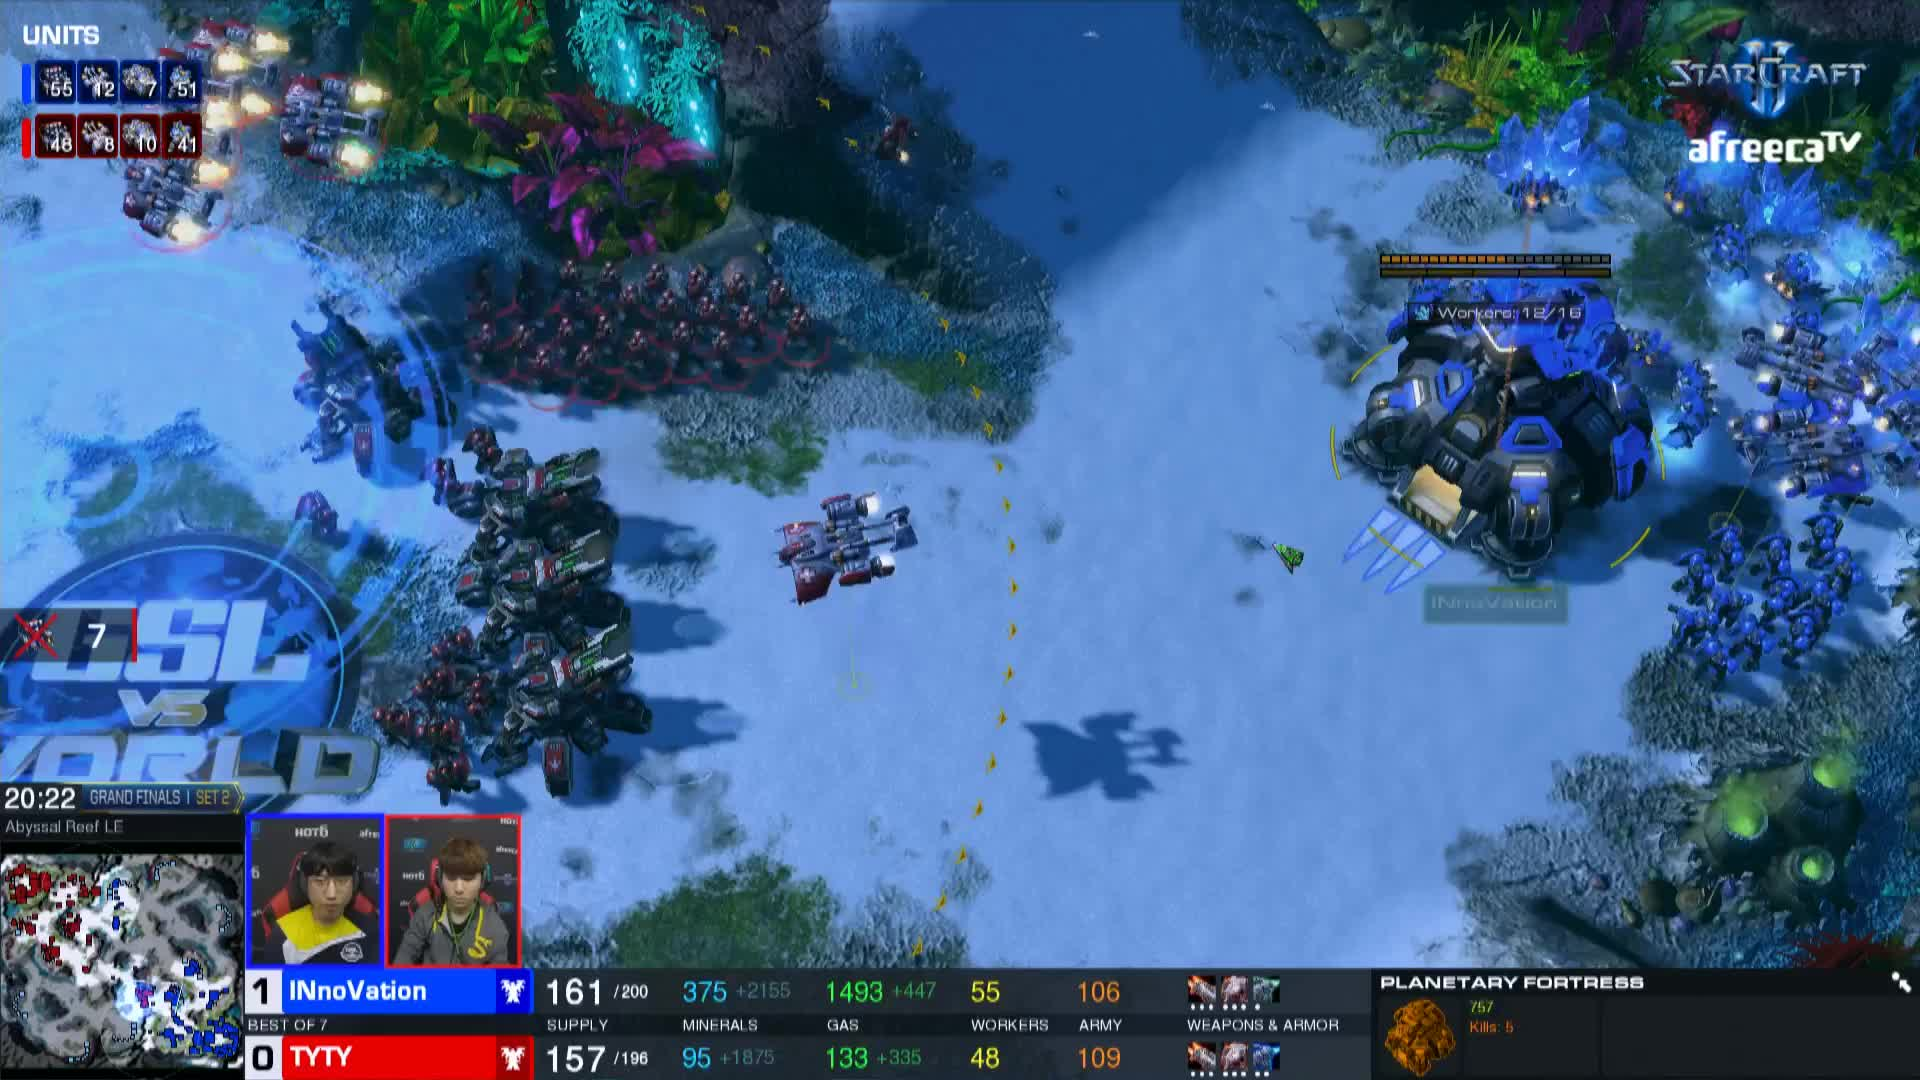
\includegraphics[width=\textwidth]{sc2}
\caption{A game of StarCraft 2. Blue player must constantly switch between defending his resource gathering units from red player’s army and at the same time coordinating an attack of his own, seen on the minimap in bottom left. 
Source: Global StarCraft League tournament “GSL vs the World”, August 2017}
\label{fig:sc2}
\end{center}
\end{figure}

\noindent Mathematically, StarCraft II can be viewed as POMDP (see section~\ref{mdp}) with practically infinite state and action spaces.
For this reason, it is especially beneficial to rely on function approximators when attempting to navigate this environment via RL based agents.

\subsection{PySC2}

To communicate with the game programmatically, PySC2 library was used. This library exposes a list of spatial and non-spatial features containing information similar to what a player would have access to. All benchmark results were gathered on a set of minigames: maps with pre-defined sets of goals such as moving a unit to a target location, defeating enemy army or gathering resources and building structures (Figure \ref{fig:pysc2}). Full specification for input features and actions can be viewed online: \url{https://github.com/deepmind/pysc2/blob/master/docs/environment.md}

\begin{figure}[ht]
\begin{center}
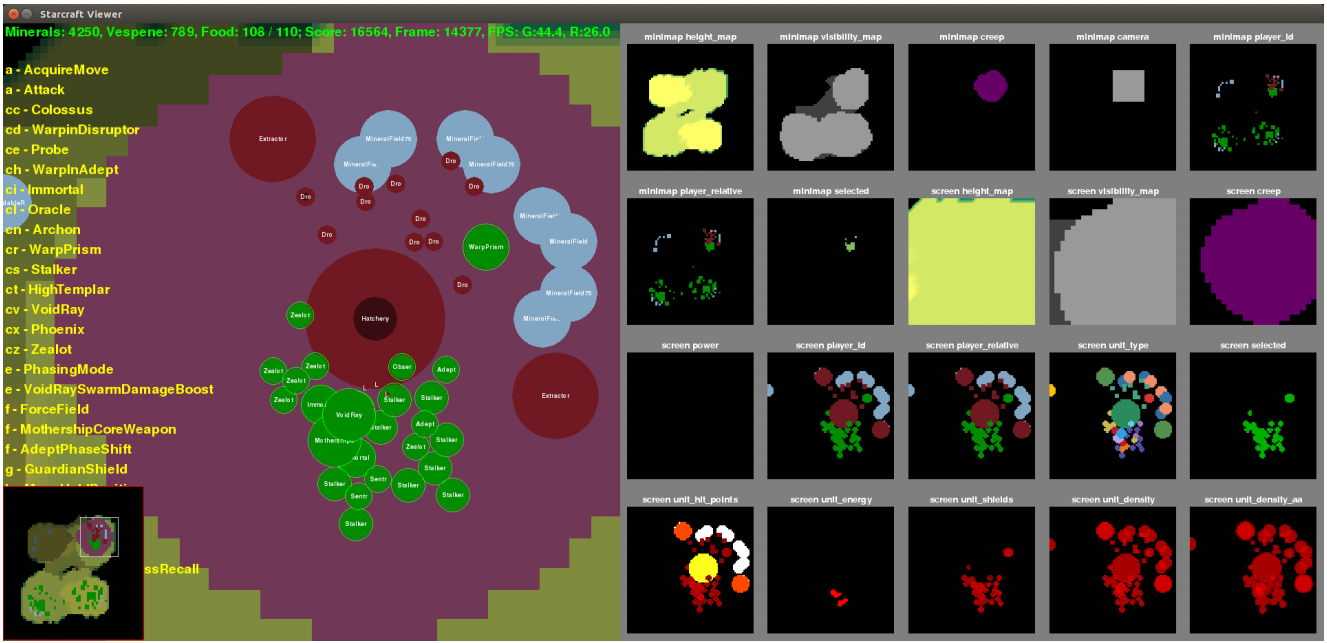
\includegraphics[width=\textwidth]{pysc2}
\caption{PySC2 environment view example. On the left is a simplified game engine GUI meant to illustrate what is happening in the game for a human observer. On the right are the actual spatial features an AI agent would see, including unit and structure affiliation, types, health and visibility~\cite{Vinyals2017}.}
\label{fig:pysc2}
\end{center}
\end{figure}